\chapter{Implementación}

En este capítulo se desarrolla de manera profunda la implementación de cada uno de los módulos que componen el software. Se incluyen las características de cada uno de ellos, tipos de estructuras creadas, toma de decisiones, flujos de trabajo y algunos ejemplos de uso.

En la primera sección se define y se explica cómo se ha estructurado todo el software desarrollado, incidiendo en cada uno de las soluciones individuales que lo componen. Tras eso se hace un repaso al desarrollo de la interfaz de usuario. Finalmente se desarrolla el despliegue del software usando contenedores de Docker, además de un ejemplo de despliegue en producción.


\section{Estructura del software creado}

Como se introducía en el capítulo \hyperref[cap:5]{cinco}, el software se basa en una arquitectura de microservicios. Estos son tres, siendo dos de ellos esenciales y uno opcional. Los principales son el \textit{backend} y los \textit{workers}, y el tercero es el \textit{frontend}, la interfaz de usuario.

Centrándonos en la parte de procesamiento de datos, es decir, \textit{backend} y \textit{workers}, debido a las características de los datos que ambos microservicios manejan estos, se han creado tres componentes para implementarlos. Cuando se trata de desarrollo de software haciendo uso de \textit{.NET} y \textit{C\#}, el software se suele organizar en proyectos y soluciones.

Un proyecto contiene todos los archivos necesarios (de cualquier tipo) que componen un archivo ejecutable o una biblioteca. Además, incluye toda aquella configuración necesaria para que pueda ser compuesto, compilado o utilizado (como podrían ser por ejemplo dependencias de otros proyectos).

Por otro lado, una solución es una composición de proyectos. Es un contenedor que, junto con cierta configuración, relaciona distintos proyectos para crear un software.

En el caso de \textbf{Matroos} se han creado tres soluciones. Estas son:

\begin{itemize}
	\item \textbf{\textit{Matroos.Resources}}. Contiene todos los servicios, clases y otros recursos compartidos. Actúa como librería de recursos compartidos para las otras soluciones.
	\item \textbf{\textit{Matroos.Backend}}. Solución compuesta por el proyecto \textit{Matroos.Backend} y la librería \textit{Matroos.Resources}.
	\item \textbf{\textit{Matroos.Worker}}. Solución compuesta por el proyecto \textit{Matroos.Worker} y la librería \textit{Matroos.Resources}.
\end{itemize}

En el siguiente cuadro se puede observar la estructura de los directorios de las soluciones y proyectos, y corresponde con la estructura usual que se sigue a la hora de crear soluciones en con \textit{.NET} y \textit{C\#}. Se puede observar que:

\begin{itemize}
	\item Cada solución y cada proyecto se encuentra en un directorio distinto.
	\item Las soluciones cuentan con un archivo con extensión \textit{*.sln} que define cómo se relacionan los proyectos que componen dicha solución.
	\item Cada proyecto cuenta con un archivo de extensión \textit{*.csproj} que contiene las dependencias y otros parámetros que definen cómo debe construirse ese proyecto.
	\item Existen proyectos adicionales para pruebas unitarias y de integración, para asegurar el correcto funcionamiento del software.
\end{itemize}

\begin{lstlisting}[style=tree]
Matroos
│
├── resources
│   ├── Matroos.Resources.sln
│   ├── src
│   │   └── Matroos.Resources
│   │       └── Matroos.Resources.csproj
│   └── tests
│       └── Matroos.Resources.Tests
│
├── backend
│   ├── Matroos.Backend.sln
│   ├── src
│   │   └── Matroos.Backend
│   │       └── Matroos.Backend.csproj
│   └── tests
│       └── Matroos.Backend.Tests
│           └── Matroos.Backend.Tests.csproj
│
└── worker
│   ├── Matroos.Worker.sln
│   ├── src
│   │   └── Matroos.Worker
│   │       └── Matroos.Worker.csproj
│   └── tests
│       └── Matroos.Worker.Tests
│           └── Matroos.Worker.Tests.csproj
│
└── frontend
\end{lstlisting}

En las siguientes secciones se desarrollan en profundidad cada uno de estos elementos.









\section{Recursos}

Esta solución actúa como librería de recursos compartidos, y contiene las clases, servicios y otros componentes que son esenciales para construir los microservicios deseados.

\subsection{Almacenamiento de datos}

En el capítulo de herramientas y diseño técnico de \textbf{Matroos} se introducía que el sistema gestor de base de datos es \textit{MongoDB}. Para acomodar este sistema, se han desarrollado distintos elementos que permiten trabajar de manera muy sencilla con este sistema gestor.

El acceso a base de datos en \textbf{Matroos} se compone de dos elementos, una interfaz para identificar los elementos a almacenar, y un servicio que ofrece las operaciones para manejar estos datos.

\subsubsection{IBaseItem.cs}

Esta interfaz es muy sencilla y cuenta con un único método estático.

\begin{lstlisting}[language=java]
public interface IBaseItem
{
    public static string CollectionName { get; } = string.Empty;
}
\end{lstlisting}

Esta interfaz es la que tienen que implementar todas aquellas clases de las que se quieren almacenar datos. En el caso de \textbf{Matroos}, puesto que sólo es necesario almacenar los bots y los comandos, sólo estas clases implementan esta interfaz.

El único método mencionado se llama \textit{CollectionName}, y corresponde con el nombre de la colección de \textit{MongoDB} donde se quieren almacenar los datos. Más información en la siguiente \hyperref[sec:datacontextservice]{sección}.

\medskip

\textbf{Flujo de trabajo}

El uso de esta interfaz es muy sencillo, en el siguiente ejemplo se ve cómo se ha definido la clase \textit{Bot}. Se puede observar que al implementar esta interfaz se define un valor para el método \textit{CollectionName}, y además se han agregado algunos decoradores para hacerle saber a \textit{MongoDB} cómo serializar y deserializar algunos campos.


\pagebreak

\begin{lstlisting}[language=java]
public class Bot : IBaseItem
{
    public static string CollectionName { get; } = "bots";

    [BsonId]
    [BsonRepresentation(BsonType.String)]
    public Guid Id { get; set; }
    
    [BsonElement("name")]
    public string Name { get; set; }
    
    // El resto de elementos se ha omitido.
}
\end{lstlisting}

\subsubsection{DataContextService.cs}
\label{sec:datacontextservice}


Este servicio es el que permite realizar operaciones con los datos almacenados en \textit{MongoDB}. Sus operaciones se definen en la interfaz \textit{IDataContextService.cs}, son las siguientes:

\begin{lstlisting}[language=java]
public interface IDataContextService
{
    public IMongoCollection<TValue>? GetCollection<TValue>() where TValue : IBaseItem;

    public Task<List<TValue>> Filter<TValue>(Expression<Func<TValue, bool>> filter) where TValue : IBaseItem;

    public Task<List<TValue>> GetAll<TValue>() where TValue : IBaseItem;

    public Task<TValue?> Get<TValue>(Guid guid) where TValue : IBaseItem;

    public Task<bool> Insert<TValue>(TValue item) where TValue : IBaseItem;

    public Task<bool> Update<TValue>(Guid guid, TValue item) where TValue : IBaseItem;

    public Task<bool> Delete<TValue>(Guid guid) where TValue : IBaseItem;
}
\end{lstlisting}

\begin{itemize}
	\item \textit{GetCollection}. Obtiene la colección asociada a ese tipo de dato, haciendo uso del método \textit{CollectionName}. Este método suele usarse de forma interna en el servicio, pero en caso necesario podría usarse para acceder a funcionalidades extra que ofrece \textit{MongoDB}.
	\item \textit{Filter}. Devuelve una lista de elementos que cumplen la condición que se indica como parámetro.
	\item \textit{GetAll}. Devuelve una lista con todos los elementos.
	\item \textit{Get}. Devuelve el elemento cuyo identificador coincide con el indicado como parámetro.
	\item \textit{Insert}. Inserta un elemento.
	\item \textit{Update}. Actualiza un elemento.
	\item \textit{Delete}. Borra un elemento.
\end{itemize}

Tanto en \textit{.NET} como en otros frameworks, existe la inyección de dependencias, que permite que ciertas dependencias sean suministradas de manera automática, en lugar de que el usuario tenga que crear los objetos necesarios de manera manual. Los servicios son un gran ejemplo de dependencias que se suelen inyectar, en el caso de aplicaciones \textit{.NET} pueden incluirse de distintas maneras, son:

\begin{itemize}
	\item \textit{Singleton}. Se crea una sola instancia para toda la aplicación. Se crea un objeto y se reutiliza para todas las llamadas a esta dependencia.
	\item \textit{Scoped}. Con ámbito. Se crea una instancia cada vez que se hace una petición al sistema, y esta instancia se reutiliza mientras se requiera el uso de la dependencia.
	\item \textit{Transient}. Cada vez que se requiere la dependencia, se crea un objeto nuevo.
\end{itemize}

En el caso del servicio de acceso a datos (\textit{DataContextService}), se ha agregado como \textit{Singleton}, de modo que sólo hay una instancia en toda la aplicación. Esto podría parecer que supone un problema, pero no es así, ya que las conexiones con la base de datos se manejan de manera interna por el conector de \textit{MongoDB} con \textit{.NET} de manera eficiente.


\medskip 

\textbf{Flujo de trabajo}

En este caso el flujo de trabajo también es sencillo. Debido a las restricciones aplicadas no es posible utilizar este servicio para manejar datos que no sean del tipo adecuado. Un ejemplo de uso es el siguiente, y muestra como se obtienen datos de MongoDB haciendo uso del servicio \textit{DataContextService} dentro de otro servicio:

\begin{lstlisting}[language=java]
public class BotsService : IBotsService
{
    private readonly IDataContextService _dataContextService;

	// Dependency injection.
    public BotsService(IDataContextService dataContextService)
    {
        _dataContextService = dataContextService;
    }
    
    public async Task<bool> UpdateBot(Bot bot)
    {
        Bot? found = await _dataContextService.Get<Bot>(bot.Id);
        if (found == null)
        {
            return false;
        }

        // Update the bot.
        found.Update(bot);

        // Push the changes to DB.
        return await _dataContextService.Update(found.Id, found);
    }
    
    // El resto de elementos se ha omitido.
}
\end{lstlisting}





\subsection{Bots}

La ejecución de bots de Discord tiene una serie de implicaciones que se han simplificado al máximo posible en el menor número de elementos. Esencialmente, las distintas librerías utilizadas permiten crear una aplicación que encapsula toda la funcionalidad de este bot de manera aislada, de modo que es posible crear distintas aplicaciones (o bots) y ejecutarlos de manera independiente.

Los componentes necesarios para crear un bot se han encapsulado dentro de la clase \textit{Bot}, y sus propiedades son las siguientes:

\begin{itemize}
	\item Identificador. Único para cada bot.
	\item Nombre. Único para cada bot.
	\item Descripción. Breve descripción del bot.
	\item \textit{Key}. Clave utilizada para acceder a la \textit{API} de \textit{Discord} a través de su cliente.
	\item Prefijo. Elemento utilizado para invocar los comandos.
	\item Comandos. Comandos configurados en el bot.
	\item Cliente de \textit{Discord}. Cliente que permite el acceso al \textit{API} de \textit{Discord}.
	\item Aplicación. La aplicación en sí que se puede ejecutar para lanzar el bot.
	\item Servicio cron. Servicio que permite ejecutar tareas en segundo plano. Más información en las siguientes secciones.
\end{itemize}

Esta clase cuenta con distintos métodos, para crear una aplicación, para lanzarla y para parar su ejecución. El más interesante es el primero de ellos, que es el siguiente:

\begin{lstlisting}[language=java]
public (IHost, CronService) GenerateRunnable()
{
    CronService cron = new(this);

    IHost app = Host
        .CreateDefaultBuilder()
        .ConfigureLogging(logging =>
        {
            // Logging to be configured.
        })
        .ConfigureDiscordShardedHost((HostBuilderContext context, DiscordHostConfiguration config) =>
        {
            config.SocketConfig = new DiscordSocketConfig
            {
                LogLevel = LogSeverity.Verbose,
                AlwaysDownloadUsers = false,
                MessageCacheSize = 200,
                TotalShards = 4
            };

            config.Token = Key;
        })
        .ConfigureServices((_, services) =>
        {
            services
                // Add the Bot instance as a singleton service.
                .AddSingleton(this)

                // Add the command handler as a hosted service.
                .AddHostedService<CommandHandler>()

                // Add the CronService as a singleton service.
                .AddSingleton(cron);
        })
        .Build();

    return (app, cron);
}
\end{lstlisting}

Si se observa detenidamente se puede observar que se está generando una aplicación muy similar a una aplicación de \textit{.NET} usual, de hecho se hace uso de la interfaz \textit{IHost}, que es una abstracción para crear aplicaciones.

Por otro lado, se configuran algunos servicios, son el bot a utilizar dentro de esa aplicación, el \textit{CommandHandler} y el servicio \textit{Cron}.

Una vez esta aplicación es creada se puede ejecutar a voluntad del usuario.

\subsubsection{\textit{CommandHandler}}

Este elemento es la capa que se interpone entre el mensaje que envía un usuario para ejecutar un comando, y la ejecución de ese comando. Este \textit{handler} (o manejador) se ha diseñado de tal manera que sea compatible con cualquier combinación de comandos de cualquier tipo de bot.

La funcionalidad principal de este elemento se encuentra en el siguiente método, el cual es bastante sencillo. Analiza los mensajes que mandan los usuarios, y determina si deben ser ejecutados o no.

\begin{lstlisting}[language=java]
private Task OnMessageReceived(SocketMessage socketMessage)
{
    // Handle user messages only.
    if (socketMessage.Source != Discord.MessageSource.User)
    {
        return Task.CompletedTask;
    }

    string commandWithPrefix = socketMessage.Content.Split(" ").FirstOrDefault() ?? "";
    string trigger = commandWithPrefix.Replace(_bot.Prefix, "");

    UserCommand? foundCommand = _bot.UserCommands.Find(command => command.Trigger.Equals(trigger));
    if (foundCommand == null)
    {
        return Task.CompletedTask;
    }

    // Run the command (asynchronously).
    CommandHelper.RunCommand(_client, socketMessage, _bot, foundCommand);

    return Task.CompletedTask;
}
\end{lstlisting}

Una vez identificado el comando se hace uso del método \textit{RunCommand}, el cual ejecuta el comando encontrado según su tipo. Más información sobre este proceso en la siguiente sección.





\subsection{Comandos}

En esta sección se profundiza en todo el desarrollo realizado en torno a la gestión y ejecución de comandos. Se comienza por el punto más básico, los comandos ``base'', se continúa por los comandos que pueden definir los usuarios y se termina introduciendo los tipos comandos que se han implementado y otros detalles adicionales.

\subsubsection{\textit{BaseCommand}}

Como se introducía en el capítulo cinco, todo lo que está relacionado con los comandos se ha diseñado para que sea lo más reutilizable posible. Por ello se introdujo el concepto \textit{BaseCommand}, el cual es la definición más básica de un tipo de comando.

Se define por las siguientes propiedades:

\begin{itemize}
	\item AllowedModes. Los modos de ejecución del comando.
	\item CommandType. El tipo de comando.
	\item NeedsPrefix. Si el comando necesita ser invocado con un prefijo o no.
	\item Parameters. La lista de parámetros que necesita este comando para funcionar correctamente.
\end{itemize}

La definición, como se adelantaba, es muy simple. Siendo esta la forma más básica, los distintos tipos de comandos que se quieran desarrollar deberán heredar por tanto de esta clase.


\subsubsection{\textit{CustomCommands}}

Los \textit{CustomCommands} no son mas que implementaciones concretas de tipos de comandos. Estas implementaciones no están restringidas de ninguna manera, por lo que cualquier usuario podría desarrollar cualquier cualquier comando que se le ocurriese.

Un ejemplo de comando \textit{custom} podría ser el siguiente:

\begin{lstlisting}[language=java]
public class HelloCommand : BaseCommand, IRunnableCommand
{
    public HelloCommand() : base(CommandType.HELLO, true)
    {
        AllowedModes = new() { CommandMode.SINGLE };
    }

    public async Task Run(DiscordShardedClient client, SocketMessage message, Bot botSettings, UserCommand command)
    {
        await message.Channel.SendMessageAsync("Hi!").ConfigureAwait(false);
    }
}
\end{lstlisting}

Se puede observar que:

\begin{itemize}
	\item Se han definido los \textit{AllowedModes}.
	\item No se han definido parámetros, ya que este comando no los necesita.
	\item Se ha implementado la interfaz \textit{IRunnableCommand}, que fuerza a que se implemente el método \textit{Run}. Este método contiene el código que se ejecutará cuando un usuario active un comando de este tipo.
\end{itemize}

Este caso es muy sencillo, ya que al ejecutarlo sólo se devuelve el mensaje \textit{Hi!} por el cliente de \textit{Discord}, pero como se mencionaba anteriormente, las posibilidades son infinitas.


\subsubsection{\textit{UserCommand}}

Estos elementos son los que puede crear libremente un usuario, y son los que se almacenan en base de datos. Cada uno de estos objetos contiene la información necesaria para definir un comando en concreto que, además, es reutilizable entre distintos bots.

Siguiendo el caso del \textit{CustomCommand} (\textit{HelloCommand}) creado en la sección anterior, se podrían crear tantos comandos como se quisieran a partir del tipo \textit{CommandType.HELLO}. En el caso de que un comando tuviera parámetros, se pueden especificar esa serie de datos en un \textit{UserCommand} para crear distintos comandos a partir del genérico.


\subsubsection{Comandos propuestos e implementados}

En el capítulo que desarrollaba el diseño técnico se proponían cinco tipos de comandos, los cuales han sido implementados, son los siguientes:

\begin{itemize}
	\item \textbf{\textit{MessageCommand}}
	\item \textbf{\textit{PingCommand}}
	\item \textbf{\textit{StatusCommand}}
	\item \textbf{\textit{TimerCommand}}
	\item \textbf{\textit{VersionCommand}}
\end{itemize}

Del mismo modo que se mencionaba en la sección anterior, para cada uno de estos tipos se ha creado una clase que hereda de \textit{BaseCommand} e implementa la interfaz \textit{IRunnableCommand}, además de definir las distintas propiedades concretas de cada uno de ellos. Tras eso se ha implementado el método \textit{Run}, que permite que el comando pueda ser ejecutado.

Las implementaciones concretas se pueden consultar en \href{https://github.com/harvestcore/matroos/tree/develop/resources/src/Matroos.Resources/Classes/Commands/CustomCommands}{el repositorio} del proyecto en \textit{GitHub}.

Volviendo a la ejecución de comandos, en la sección \textit{Bots} anterior se mencionaba que los comandos se ejecutaban haciendo uso del método \textit{RunCommand}, este tiene la siguiente forma:

\begin{lstlisting}[language=java]
public static void RunCommand(DiscordShardedClient client, SocketMessage message, Bot bot, UserCommand command)
{
    // Get the command attribute.
    CommandAttribute attribute = command.Type.GetAttribute<CommandAttribute>();
    Type commandType = attribute.Command;

    if (commandType == null)
    {
        throw new InvalidDataException("Missing command type");
    }

    // Generate an instance from the command type.
    object? generatedInstance = Activator.CreateInstance(attribute.Command);

    // Invoke the "Run" method to run the command.
    commandType
        .GetMethod("Run")
        ?.Invoke(generatedInstance, new object[] { client, message, bot, command });
}
\end{lstlisting}

En esencia, cuando se quiere ejecutar un comando se sigue el siguiente proceso:

\begin{enumerate}
	\item Se identifica el tipo de comando que se quiere ejecutar.
	\item Se obtiene la clase que implementa ese tipo comando.
	\item Se hacen comprobaciones previas para evitar errores.
	\item Se ejecuta el método \textit{Run} con los parámetros necesarios.
\end{enumerate}

Este modelo de abstracción permite la separación de dos elementos que a priori pueden parecer que deben estar relacionados de una manera más fuerte. Por un lado se encuentra la funcionalidad específica de los comandos, y por otro se almacena la configuración concreta para cada caso de uso. Esto permite que se pueda reutilizar el código de estos comandos y además se simplifica la cantidad de datos a almacenar.


\subsubsection{Utilidades}

De manera adicional (y necesaria) se han definido algunos enumerados y clases necesarios para poder confeccionar esta estructura. Son:

\begin{itemize}
	\item \textit{CommandMode}. Para definir los modos de ejecución de los comandos.
	\item \textit{CommandSignature}. Para encapsular la configuración de un tipo de comando.
	\item \textit{CommandType}. Para definir los tipos de comando.
	\item \textit{ParameterSignature}. Para encapsular cada uno de los parámetros que puede tener un comando.
	\item \textit{DataType}. Para definir los tipos de datos de los parámetros.
\end{itemize}

También se han definido decoradores que permiten agregar funcionalidad extra a los distintos enumerados, además de diversas funciones auxiliares.


\subsubsection{Procesamiento en segundo plano}

El procesamiento en segundo plano es la característica principal del comando de tipo \textit{TIMER}. Este comando permite ejecutar otro comando de manera reiterativa cuando se cumple un lapso de tiempo definido por una expresión \href{https://docs.oracle.com/cd/E12058_01/doc/doc.1014/e12030/cron_expressions.htm}{\textit{cron}}.

Se ha utilizado la librería \href{https://www.quartz-scheduler.net/}{\textit{Quartz}}, que permite acceder a un planificador que posibilita la ejecución de tareas de manera transparente para el usuario.

Principalmente la interacción con el planificador se hace dentro del servicio \textit{CronService}, el cual se encuentra en cada instancia de cada bot que se ejecuta en el sistema. Este servicio accede a todos los comandos de tipo \textit{TIMER} que se encuentran configurados en los bots, y los ejecuta en segundo plano teniendo en cuenta el intervalo \textit{cron} de cada uno de ellos.

Esta ejecución de los comandos se produce de manera muy similar a la explicada en secciones anteriores. Se ha definido un trabajo (\textit{RunCommandJob}) que se encarga de esta ejecución. Es el siguiente:

\begin{lstlisting}[language=java]
public class RunCommandJob : IJob
{
    public Task Execute(IJobExecutionContext context)
    {
        if (context == null)
        {
            return Task.CompletedTask;
        }

        // Extract the parameters.
        UserCommand? timerCommand = context.MergedJobDataMap?.Get("Command").GetValue<UserCommand>();
        Bot? bot = context.MergedJobDataMap?.Get("Bot").GetValue<Bot>();

        if (timerCommand == null || bot == null || bot.Client == null)
        {
            return Task.CompletedTask;
        }

        // The command to be executed.
        string? commandToExecute = timerCommand.Parameters["CommandId"].GetValue<string>();
        UserCommand? commandFound = bot.UserCommands.Find(command => command.Id == Guid.Parse(commandToExecute ?? ""));

        if (commandFound == null || commandFound.Mode == CommandMode.INLINE || commandFound.Mode == CommandMode.HEADLESS)
        {
            return Task.CompletedTask;
        }

        // Run the command.
        CommandHelper.RunCommand(bot.Client, null, bot, commandFound);

        return Task.CompletedTask;
    }
}
\end{lstlisting}

El único detalle a tener en cuenta es que en este contexto el comando no es ejecutado tras el mensaje de un usuario solicitando su ejecución, por lo que en este caso el mensaje es nulo (línea 29).


\subsection{Servicios}

Además del servicio de acceso a base de datos descrito en secciones anteriores, se ha desarrollado otro servicio que ayuda a la configuración del software. Este es el \textit{ConfiguracionService} y actúa como gestor de configuraciones.

Permite:

\begin{itemize}
	\item Obtener variables de entorno.
	\item Obtener variables de configuración del archivo \textit{appsettings.json}, usual en aplicaciones de \textit{.NET} y \textit{C\#}.
	\item Crear nuevas variables de configuración.
\end{itemize}


\subsubsection{Utilidades API REST}

Con el fin de simplificar la implementación se han creado elementos adicionales, como por ejemplo distintos modelos para devolver de manera uniforme los datos en los \textit{endpoints}. Estos son:

\begin{itemize}
	\item \textit{SuccessResponse}, que cuenta con un atributo \textit{Success} que indica si una operación se ha realizado correctamente o no.
	\item \textit{ItemsResponse}, que cuenta con los atributos \textit{Count} e \textit{Items}. El primero indica cuantos elementos se están devolviendo, y el segundo es un array con dichos elementos.
\end{itemize}


\subsection{Otros elementos}

Además, se han desarrollado distintas utilidades para simplificar las tareas de \textit{testing}, como son:

\begin{itemize}
	\item Clase \textit{BaseTest}, que encapsula y configura la conexión de base de datos para un entorno de pruebas. Además de incluir un método para vaciar una colección en concreto.
	\item Clase \textit{Sample}, modelo de datos sencillo usado para ciertas pruebas.
	\item Clase \textit{TestHelper}, que contiene métodos de extensión para facilitar las pruebas de \textit{endpoints} y otros elementos.
\end{itemize}

También se han implementado \textit{mappers} de datos debido a que en base de datos los comandos configurados en los bots se almacenan como una lista de identificadores y es mucho más cómodo trabajar con objetos de tipo \textit{UserCommand}.

Estos permiten que, cuando se cargan bots desde base de datos, la lista de identificadores se convierta en una lista de \textit{UserCommand}; y del mismo modo, cuando se quiere almacenar un bot en base de datos, esta lista de \textit{UserCommand} se convierte en un listado de identificadores.




\section{Backend}

Este microservicio es el principal de \textbf{Matroos}, e incluye gran parte de la lógica. Se compone de una serie de servicios y controladores, además de ciertas utilidades.

\subsection{Servicios}

Se han desarrollado distintos servicios para manejar todas las operaciones y todos los datos que se registran en el \textit{backend}. En las siguientes secciones se profundiza en cada uno de ellos.

\subsubsection{\textit{BackgroundService}}

La comunicación entre el \textit{backend} y los \textit{workers} se hace a través de \textit{HTTP}, siendo el \textit{backend} el que se encarga de comunicarse con los \textit{workers} para conocer su estado. Para ello se ha creado este servicio, el cual realiza actualizaciones periódicas de los \textit{workers}.

Previa ejecución del microservicio del backend, es necesario indicar mediante variables de entorno (o en tiempo de ejecución mediante el \textit{ConfiguracionService}) las \textit{URL} de los \textit{workers} que se encuentran desplegados. Una vez estas \textit{URLs} son conocidas por el sistema y por el servicio, cada 10 segundos se realizan peticiones a estos \textit{workers}, para conocer su estado.

Es una implementación de \textit{Microsoft.Extensions.Hosting.BackgroundService}, que es el servicio básico a implementar en caso de necesitar procesamiento en segundo plano en \textit{.NET}.

\subsubsection{\textit{CommunicationService}}

Este servicio se encarga de toda la comunicación entre el \textit{backend} y los \textit{workers}. Implementa una serie de métodos que realizan las distintas llamadas \textit{HTTP} a los \textit{endpoints} de los \textit{workers}.

\subsubsection{Otros servicios}

Se han desarrollado servicios para manejar todas las operaciones relacionadas con los bots, los comandos y los workers, son:

\begin{itemize}
	\item \textit{BotsService}
	\item \textit{UserCommandsService} 
	\item \textit{WorkersService} 
\end{itemize}

\subsection{Controladores}

Del mismo modo que existen tres servicios distintos para manejar los datos del sistema, existen tres controladores que implementan los endpoints de la \textit{API REST}. Los controladores son los siguientes, y esencialmente hacen uso de los servicios anteriores, para realizar las operaciones necesarias. De forma adicional se ha creado un controlador para conocer el estado del \textit{backend}.

\begin{itemize}
	\item \textit{BotsController}
	\begin{itemize}
		\item \textit{GET /bots}
		\item \textit{GET /bots/<botId>}
		\item \textit{POST /bots}
		\item \textit{PUT /bots}
		\item \textit{DELETE /bots/<botId>}
	\end{itemize}
	\item \textit{UserCommandsController}
	\begin{itemize}
		\item \textit{GET /commands/signatures}. Permite obtener la definición de todos los tipos de comando que se pueden crear en el sistema.
		\item \textit{GET /commands}
		\item \textit{GET /commands/<commandId>}
		\item \textit{POST /commands}
		\item \textit{PUT /commands}
		\item \textit{DELETE /commands/<commandId>}
	\end{itemize}
	\item \textit{WorkersController}
	\begin{itemize}
		\item \textit{GET /workers/<workerId>/start/<botId>}
		\item \textit{GET /<workerId>/stop/<botId>}
		\item \textit{GET /workers}
		\item \textit{GET /workers/<workerId>}
		\item \textit{POST /workers/<workerId>}
		\item \textit{DELETE /workers/<workerId>}
	\end{itemize}
	\item \textit{HealthController}
	\begin{itemize}
		\item \textit{GET /health}. Para conocer el estado del \textit{backend}.
	\end{itemize}
\end{itemize}

En el anexo XXX se encuentra la especificación y documentación más completa de todos y cada uno de los endpoints del sistema.






\section{Worker}

Este microservicio es mucho mas sencillo que los otros, ya que solo se encarga de almacenar en memoria una serie de bots, los cuales puede ejecutar o parar.

\subsection{Servicios}

El único servicio implementado en este caso es el siguiente:

\begin{itemize}
	\item \textit{MainService}, administra los bots que se encuentran desplegados en el \textit{worker}.
\end{itemize}

\subsection{Controladores}

En este caso también es sencilla la implementación, y solo han sido necesarios dos controladores.

\begin{itemize}
	\item \textit{MainController}
	\begin{itemize}
		\item \textit{GET /}
		\item \textit{POST /}
		\item \textit{PUT /}
		\item \textit{DELETE /<botId>}
		\item \textit{GET /start/<botId>}
		\item \textit{GET /stop/<botId>}
	\end{itemize}
	\item \textit{HealthController}
	\begin{itemize}
		\item \textit{GET /health}. Para conocer el estado del \textit{worker}.
	\end{itemize}
\end{itemize}





\section{Frontend}

El \textit{frontend} que se ha implementado es una de las infinitas posibles propuestas que se pueden desarrollar. En las siguientes secciones se detallan los módulos y componentes que se han desarrollado.

\subsection{Componentes}

Se han intentado reutilizar lo máximo posible los componentes de la interfaz de usuario. Para ello se han identificado los más relevantes, son:

\begin{itemize}
	\item \textit{SimpleTable}. Tabla sencilla con paginación que permite mostrar una serie de datos con columnas y acciones definidas por el usuario.
	\item \textit{CollapsibleTable}. Tabla similar a la anterior, cuya diferencia reside en que cada fila muestra otra tabla.
	\item \textit{ChipSelector}. Selector de elementos en formato \textit{``chip''}. Utilizado para seleccionar los comandos dentro de un bot.
	\item \textit{ConfirmationDialog}. Diálogo sencillo de confirmación de acciones.
\end{itemize}

Además de estos, se han desarrollado otros componentes, como son elementos modales para crear y editar bots, comandos y workers, o tarjetas para mostrar cierta información del sistema.

En cuanto a comunicación con el \textit{backend} se han creado una serie de funciones que permiten realizar todas las posibles acciones, como son crear, editar o eliminar bots y comandos. Así mismo se han definido una serie de tipos para identificar los distintos de datos en cada componente, función y método.

\subsection{Páginas}

Se divide en 4 páginas principales. En general, en la mayoría de ellas se ha optado por un diseño sencillo basado en listados, pues es una manera sencilla de visualizar la información. Se han utilizado componentes modales para la modificación de todos los datos del sistema.

\subsubsection{Home}

Contiene tres tarjetas con información del estado general del sistema.

\begin{figure}[H]
	\centering
	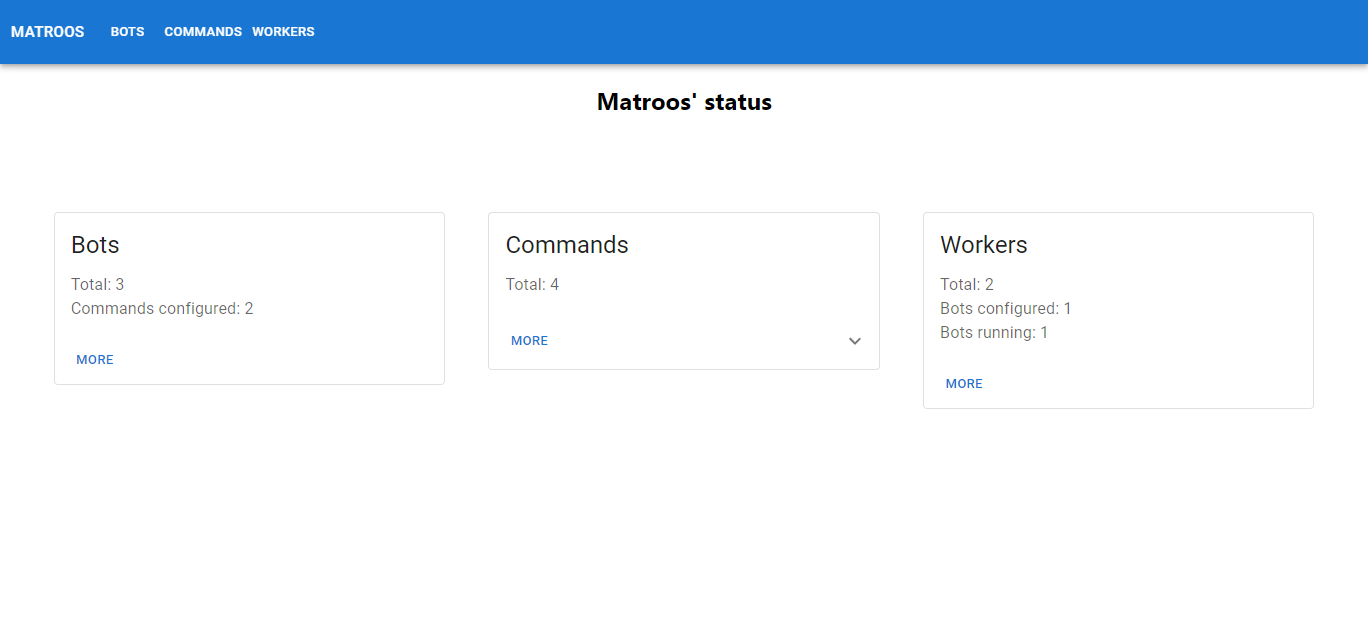
\includegraphics[width=1\textwidth]{img/front/page-home.png}
	\caption{Página principal de \textbf{Matroos}.}
\end{figure}

\subsubsection{Bots}

Listado de los bots disponibles, junto con modales para crear y editar bots.

\begin{figure}[H]
	\centering
	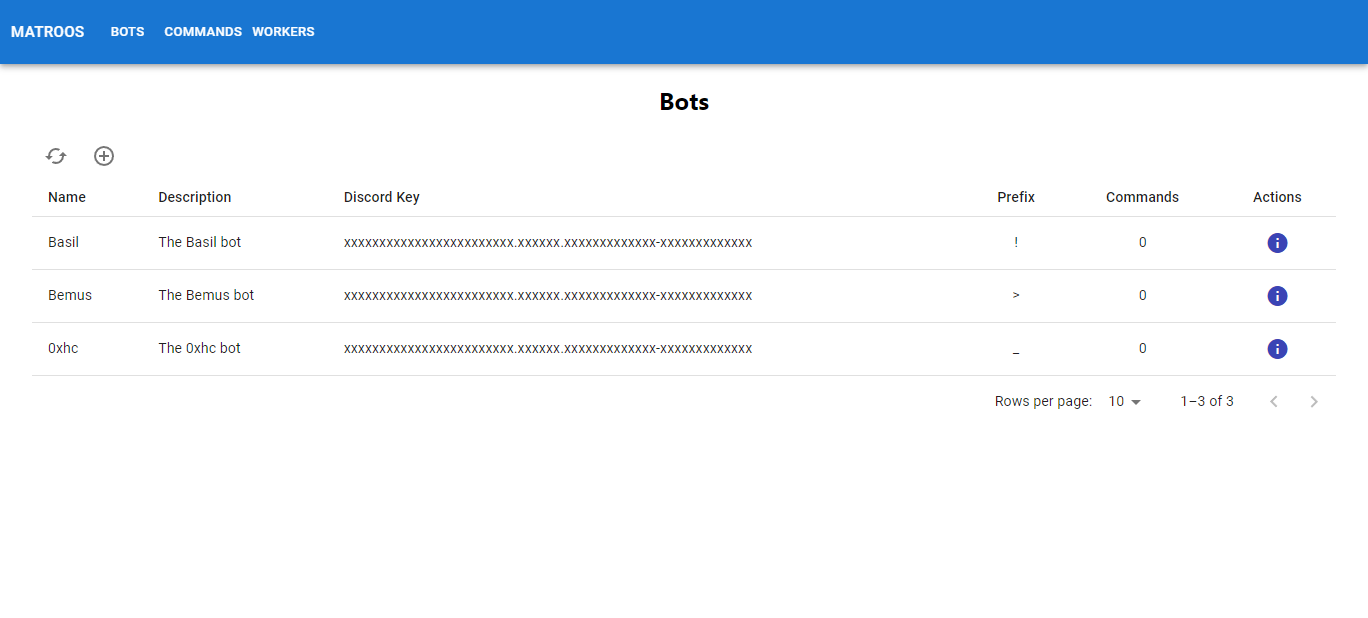
\includegraphics[width=1\textwidth]{img/front/page-bots.png}
	\caption{Página de visualización de bots.}
\end{figure}

\begin{figure}[H]
	\centering
	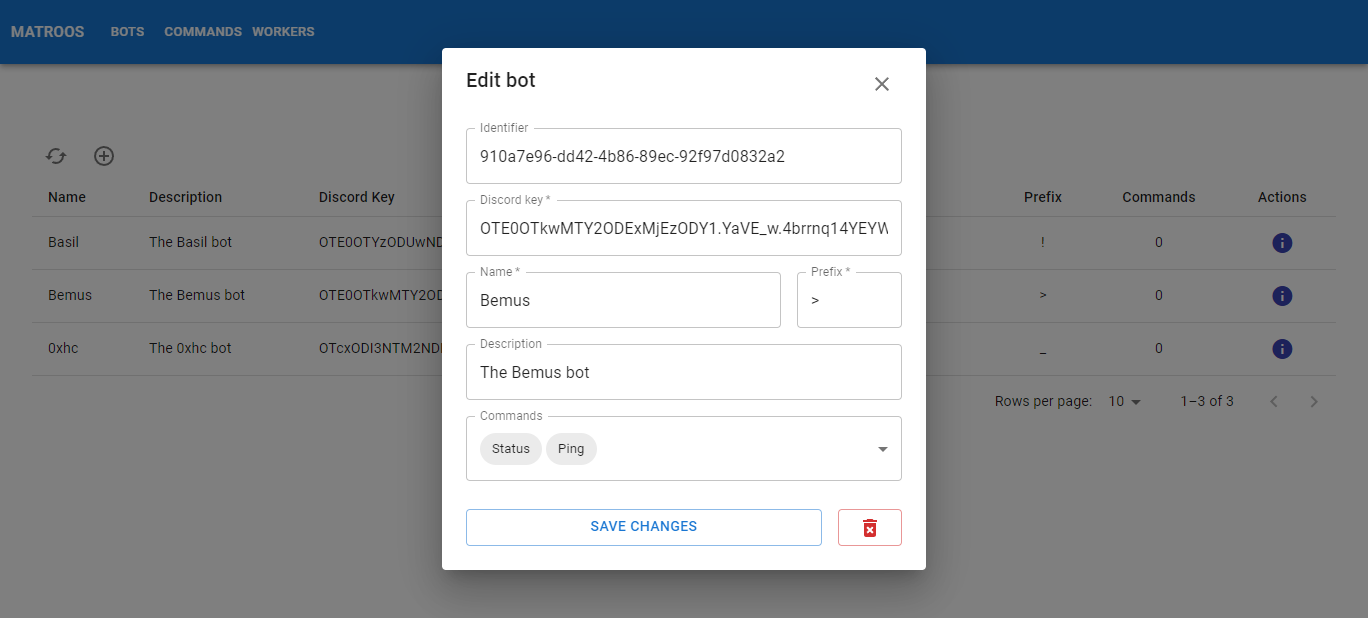
\includegraphics[width=1\textwidth]{img/front/page-bots-edit.png}
	\caption{Modal de edición de bots.}
\end{figure}

\subsubsection{Commands}

Listado de los comandos disponibles, junto con modales para crear y editar comandos.

\begin{figure}[H]
	\centering
	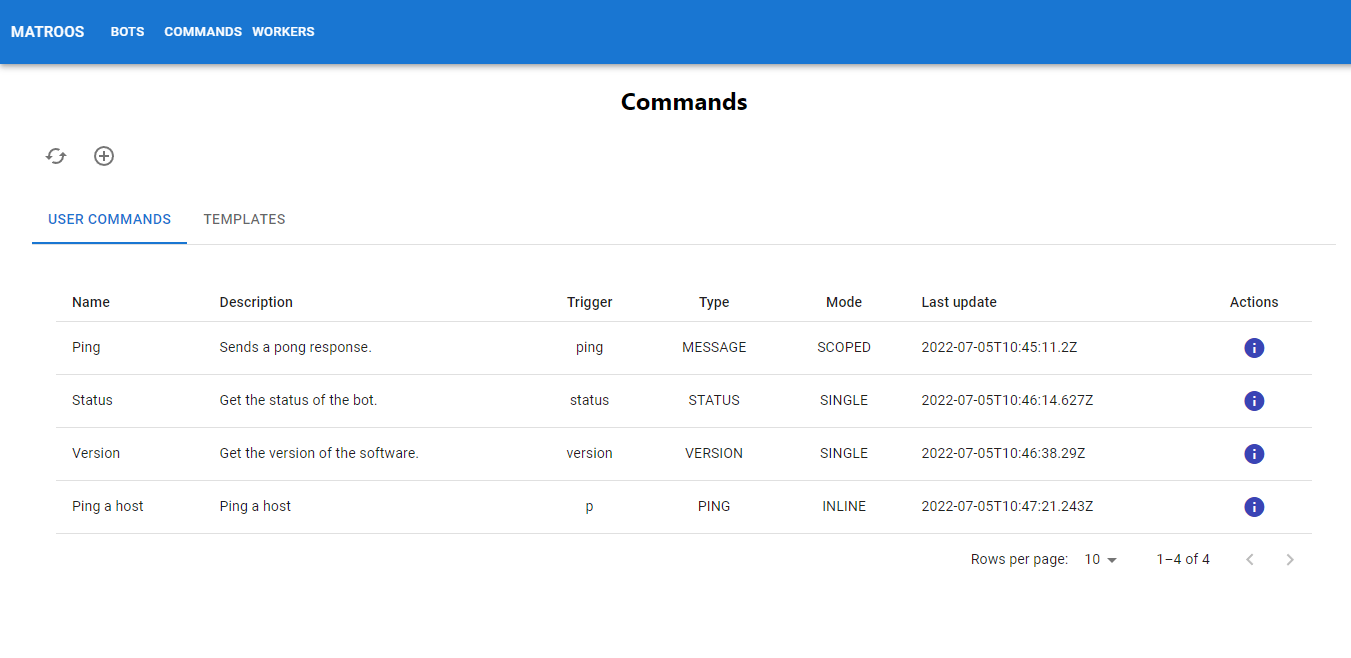
\includegraphics[width=1\textwidth]{img/front/page-commands.png}
	\caption{Página de visualización de comandos.}
\end{figure}

\begin{figure}[H]
	\centering
	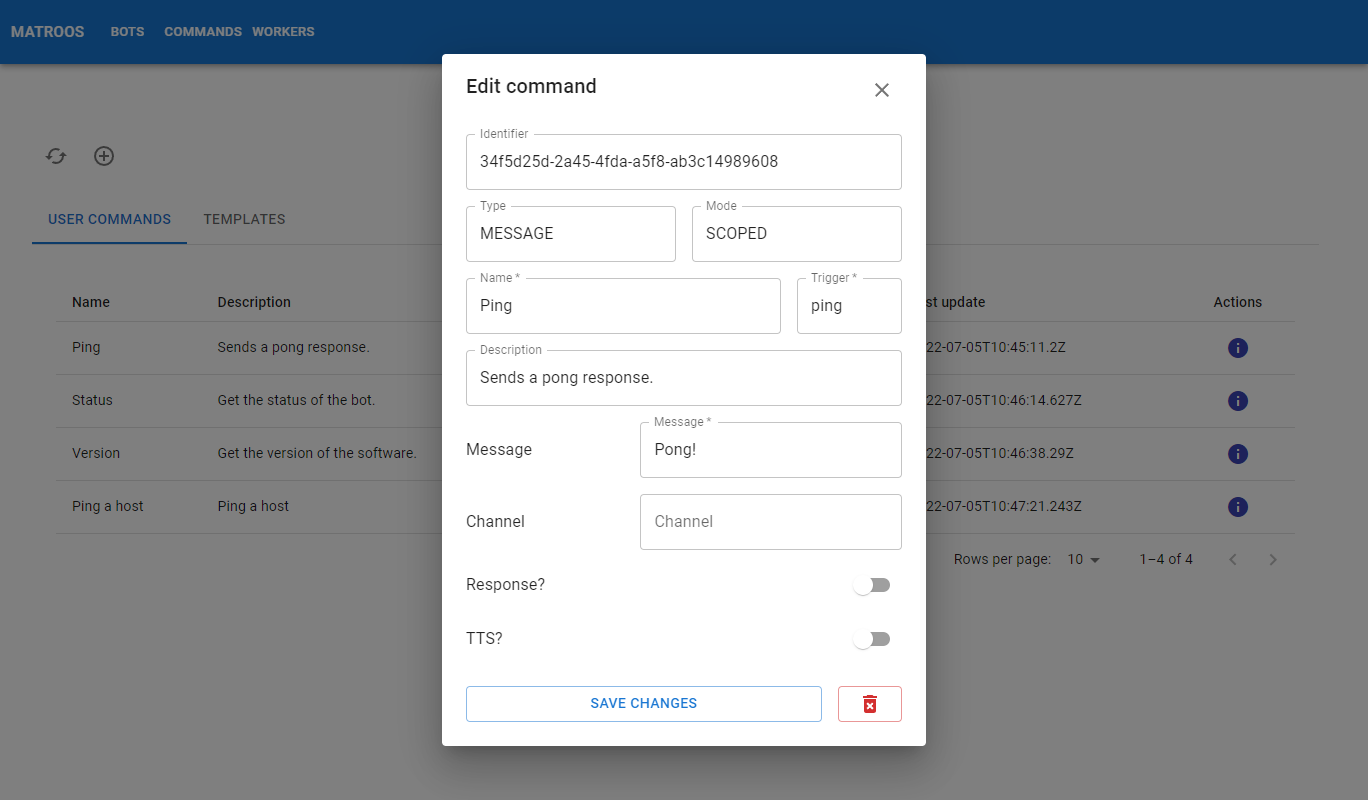
\includegraphics[width=1\textwidth]{img/front/page-commands-edit.png}
	\caption{Modal de edición de comandos.}
\end{figure}

\subsubsection{Workers}

Listado de los \textit{workers} disponibles, junto con modales para editar \textit{workers}.

\begin{figure}[H]
	\centering
	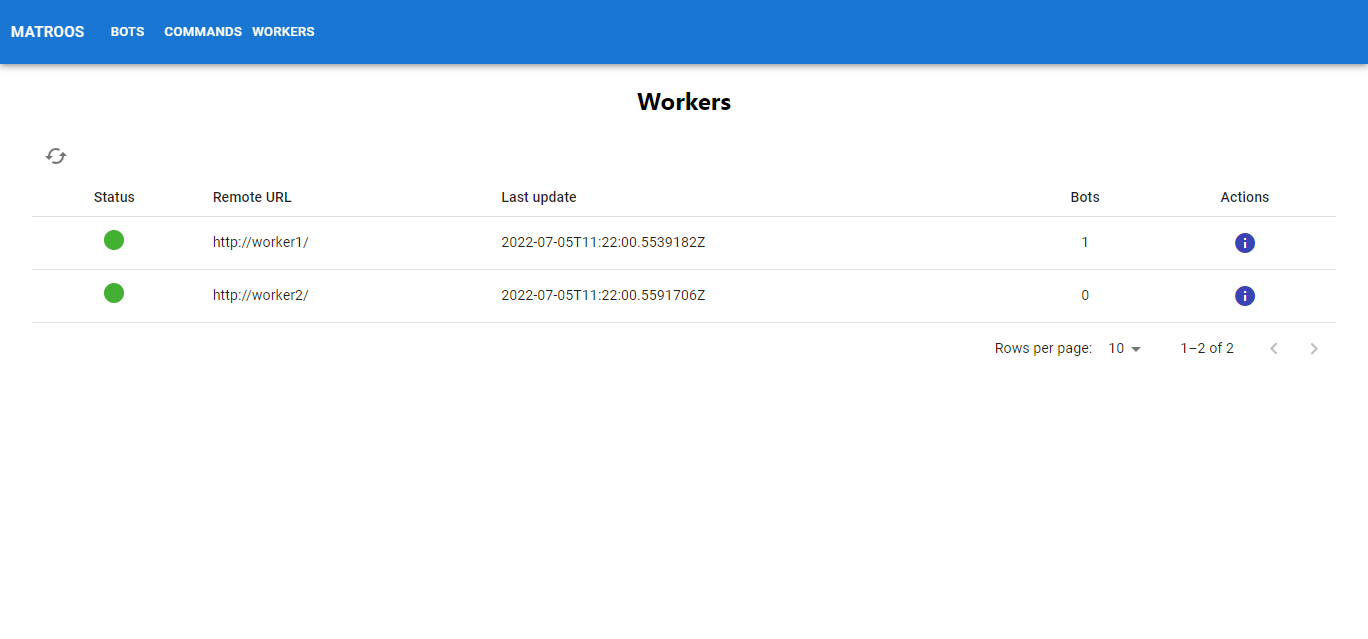
\includegraphics[width=1\textwidth]{img/front/page-workers.png}
	\caption{Página de visualización de \textit{workers}.}
\end{figure}

\begin{figure}[H]
	\centering
	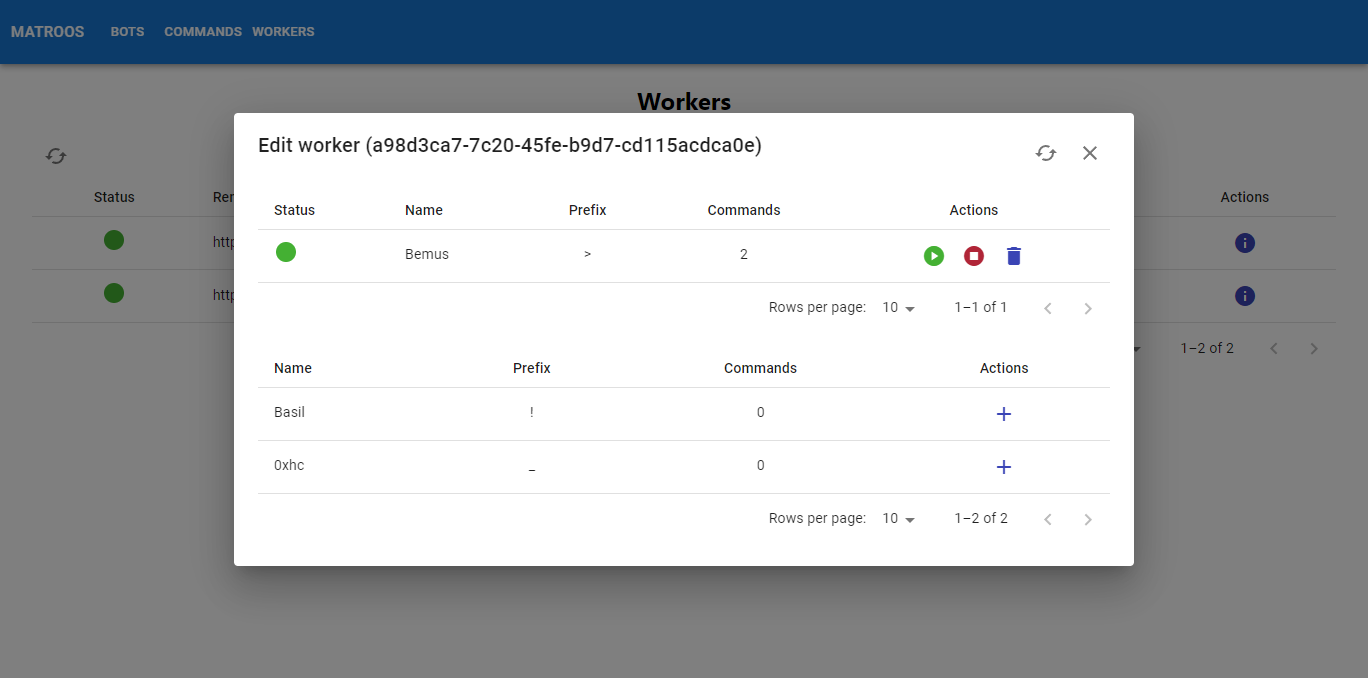
\includegraphics[width=1\textwidth]{img/front/page-workers-edit.png}
	\caption{Modal de edición de \textit{workers}.}
\end{figure}

\section{Despliegue en \textit{Docker}}

Todas los microservicios que componen \textbf{Matroos} son desplegables mediante contenedores \textit{Docker}. Para ello se han incluido archivos \textit{Dockerfile} para cada uno de ellos, además de archivos \textit{docker-compose.yml} para orquestar los servicios.

Además, cada vez que se hace una \textit{release} en \href{https://github.com/harvestcore/matroos}{el repositorio} de que contiene el código, se generan automáticamente nuevas imágenes de los microservicios \textit{backend} y \textit{worker}. Tras eso se suben al registro de imágenes que proporciona el propio \textit{GitHub}, \href{https://github.com/harvestcore?tab=packages&repo_name=matroos}{aquí}. Esto se ha configurado mediante un \textit{workflow} de \textit{GitHub Actions}, el cual puede encontrarse \href{https://github.com/harvestcore/matroos/blob/develop/.github/workflows/build-docker-images.yml}{aquí}.

Como se indicaba, se han incluido una serie de archivos \textit{Dockerfile} y \textit{docker-compose.yml}, son los siguientes:

\begin{lstlisting}[style=tree]
Matroos
│
├── Dockerfile.backend
├── Dockerfile.worker
│
├── docker-compose.override.yml
├── docker-compose.yml
│
└── frontend
    ├── Dockerfile
    └── docker-compose.yml
\end{lstlisting}

Para la confección de los siguientes archivos se han tenido en cuenta las mejores prácticas, intentando obtener imágenes lo más livianas posibles.

\begin{itemize}
	\item \textit{Dockerfile.backend}. Construye el microservicio \textit{backend}.
	\item \textit{Dockerfile.worker}. Construye el microservicio \textit{worker}.
	\item \textit{frontend/Dockerfile}. Construye el microservicio \textit{frontend}.
\end{itemize}

\begin{itemize}
	\item \textit{docker-compose.yml}. Orquesta tanto el microservicio \textit{backend} como el \textit{worker} haciendo uso de las imágenes subidas al registro de \textit{GitHub}. Además incluye la definición de un servicio de base de datos (\textit{MongoDB}).
	\item \textit{docker-compose.override.yml}. Igual que el anterior, pero en lugar de usar las imágenes del registro, construye las imágenes localmente.
	\item \textit{frontend/docker-compose.yml}. Orquesta el microservicio \textit{frontend}.
\end{itemize}


\section{Despliegue en producción}

Para realizar un despliegue en producción de podrían utilizar desde servidores domésticos como plataformas \textit{cloud} de gran complejidad. En el caso de \textbf{Matroos}, y a modo de entorno para mostrar el funcionamiento del software se ha realizado un despliegue en un servidor \textit{cloud} dedicado, se encuentra en este \href{https://0xhc.com:9000/}{enlace}.

Como se indicaba en la sección anterior, existen distintos archivos que permiten desplegar el software mediante contenedores de \textit{Docker}, y esta plataforma es la que se ha utilizado para el despliegue en producción.

La estructura de este despliegue es la siguiente:

\begin{figure}[H]
	\centering
	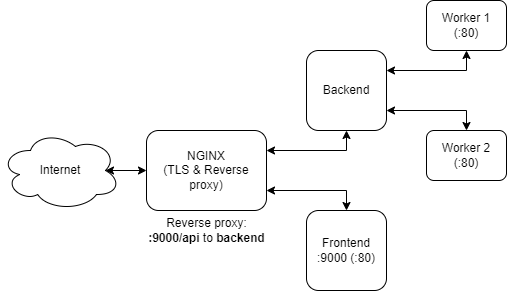
\includegraphics[width=1\textwidth]{img/production.png}
	\caption{Arquitectura del despliegue en producción.}
\end{figure}

Para conseguir esta configuración han sido necesarios algunos cambios en los archivos anteriores, además de ser necesarios algunos archivos nuevos y algunas configuraciones extra.

\subsection{Configuración de \textit{NGINX}}

El siguiente extracto muestra la configuración de un contenedor de \textit{Docker} de \textit{NGINX}.

\textbf{\textit{docker-compose.yml}}

\begin{lstlisting}[language=sh]
version: "3.3"
services:
  nginx:
    image: nginx:alpine
    container_name: nginx
    restart: always
    ports:
      - "9000:9000"   # Matroos frontend
    volumes:
      - ./nginx.conf:/etc/nginx/conf.d/default.conf
      - ./certs:/etc/nginx/certs

networks:
  default:
    external:
      name: nginx-network
\end{lstlisting}

Se puede observar que se está usando una red externa. El uso de esta permite que diferentes contenedores que se han orquestado y lanzado desde distintos archivos \textit{docker-compose.yml} compartan una misma red, y por tanto puedan comunicarse entre ellos.

\bigskip

\textbf{\textit{nginx.conf}}

\begin{lstlisting}[language=sh]
server {
    listen      9000 ssl;
    server_name 0xhc.com;

    add_header Strict-Transport-Security "max-age=31536000; includeSubDomains" always;

    error_page 497 @force_https;

    location @force_https {
        return 301 https://$host:9000$request_uri;
    }

    ssl_certificate         /etc/nginx/certs/public.crt;
    ssl_certificate_key     /etc/nginx/certs/private.key;

    location /api/ {
        auth_basic         off;
        proxy_set_header   X-Real-IP $remote_addr;
        proxy_set_header   X-Forwarded-For $proxy_add_x_forwarded_for;
        proxy_pass         http://backend/;
        proxy_http_version 1.1;
        proxy_set_header   Upgrade $http_upgrade;
        proxy_set_header   Connection "upgrade";
        add_header Strict-Transport-Security "max-age=31536000; includeSubDomains" always;
    }

    location / {
        auth_basic         off;
        proxy_set_header   X-Real-IP $remote_addr;
        proxy_set_header   X-Forwarded-For $proxy_add_x_forwarded_for;
        proxy_pass         http://matroos-front/;
        proxy_http_version 1.1;
        proxy_set_header   Upgrade $http_upgrade;
        proxy_set_header   Connection "upgrade";
        add_header Strict-Transport-Security "max-age=31536000; includeSubDomains" always;
    }
}
\end{lstlisting}

En este caso la configuración es sencilla, haciéndose un \textit{proxy} de las peticiones a los contenedores adecuados.


\subsection{Configuración de los servicios de \textbf{Matroos}}

La única modificación necesaria ha sido la agregación de la red externa compartida en los archivos \textit{docker-compose.yml}, para permitir la comunicación con el servicio de \textit{NGINX}.

\begin{lstlisting}[language=sh]
networks:
  default:
    external:
      name: nginx-network
\end{lstlisting}

Una vez se ha hecho la modificación, sólo es necesario ejecutar los contenedores, quedando así el sistema completamente desplegado.

\subsection{\textit{TLS} y seguridad}

Como se indicaba en el capítulo cinco, el sistema es inseguro, ya que no ofrece ningún tipo de autenticación. Sin embargo, también se mencionaba que hay distintas maneras de agregar capas de seguridad al sistema de manera muy sencilla con software ya existente.

Sin duda una de las más sencillas es el \textit{TLS}, y en el caso de esta configuración se ha agregado haciendo uso de un certificado proporcionado por la entidad \textit{CertBot} (\textit{Let's Encrypt}) de manera gratuita.

Además, podrían agregarse otras capas de seguridad, siendo una posible la autenticación básica (o \textit{Basic Auth}). Esta también es fácilmente configurable en \textit{NGINX} y otros sistemas. En el caso de este despliegue no se ha configurado con el fin de simplificar la configuración.
